\chapter{Lo pneumatico}
\label{Pneumatico}
%
Gli pneumatici sono probabilmente i componenti più complessi di un'auto in quanto combinano decine di elementi che devono essere formati, assemblati e combinati assieme. Il successo del prodotto finale dipende dalla loro capacità di fondersi in un prodotto coeso e che soddisfi le esigenze del conducente \cite{rill}. Essi sono caratterizzati da un comportamento altamente non lineare con una forte dipendenza da diversi fattori costruttivi e ambientali.
%
\section{Geometria}
Quando si fa riferimento ai dati puramente geometrici, viene utilizzata una forma abbreviata della notazione completa prevista dall'ente di normazione \ac{ETRTO}. Assumendo di avere uno pneumatico generico la notazione che identificherà la geometria sarà del tipo $a$ / $b$ R $c$, dove:
\begin{itemize}
	\item $a$ rappresenta larghezza nominale dello pneumatico nel punto più largo;
	\item $b$ rappresenta percentuale dell'altezza della spalla dello pneumatico in relazione alla larghezza dello stesso;
	\item $c$ rappresenta il diametro dei cerchi ai quali lo pneumatico si adatta.
\end{itemize}
Si prenda come esempio la seguente denominazione \ac{ETRTO}: 195/55R16. La larghezza nominale dello pneumatico è di circa 195 mm nel punto più largo, l'altezza della spalla corrisponde al 55\% della larghezza $-$ ovvero 107 mm $-$ e il diametro dei cerchi ai quali lo pneumatico si adatta è di 16 pollici. Con questa notazione è possibile calcolare direttamente il diametro esterno teorico dello pneumatico tramite una delle seguenti formule:
%
\begin{equation}
\phi_e = \frac{2ab}{25.4}+c \quad \text{[in]} \qquad
\end{equation}
\begin{equation}
\phi_e = 2ab+25.4c \quad \text{[mm]}
\end{equation}
%
Riprendendo l'esempio usato sopra, il diametro esterno risulterà dunque 24.44 in o 621 mm.\\
Meno comunemente usata negli USA e in Europa (ma spesso in Giappone) è la notazione che indica l'intero diametro dello pneumatico invece delle proporzioni dell'altezza della spalla laterale, quindi non secondo \ac{ETRTO}. Per fare lo stesso esempio, un cerchio da 16 pollici avrebbe un diametro di 406 mm. L'aggiunta del doppio dell'altezza dello pneumatico (2$\times$107 mm) produce un diametro totale di 620 mm. Quindi, uno pneumatico 195/55R16 potrebbe in alternativa essere etichettato come 195/620R16. Anche se queste due notazioni sono teoricamente ambigue, in pratica possono essere facilmente distinte perché l'altezza della parete laterale di uno pneumatico automobilistico è in genere molto inferiore alla larghezza. Quindi, quando l'altezza è espressa come percentuale della larghezza, è quasi sempre inferiore al 100\% (e certamente meno del 200\%). Al contrario, i diametri degli pneumatici del veicolo sono sempre superiori a 200 mm. Pertanto, se il secondo numero è superiore a 200, allora è quasi certo che viene utilizzata la notazione giapponese, se è inferiore a 200 allora viene utilizzata la notazione USA/europea.

\begin{figure}[h]
	\centering
	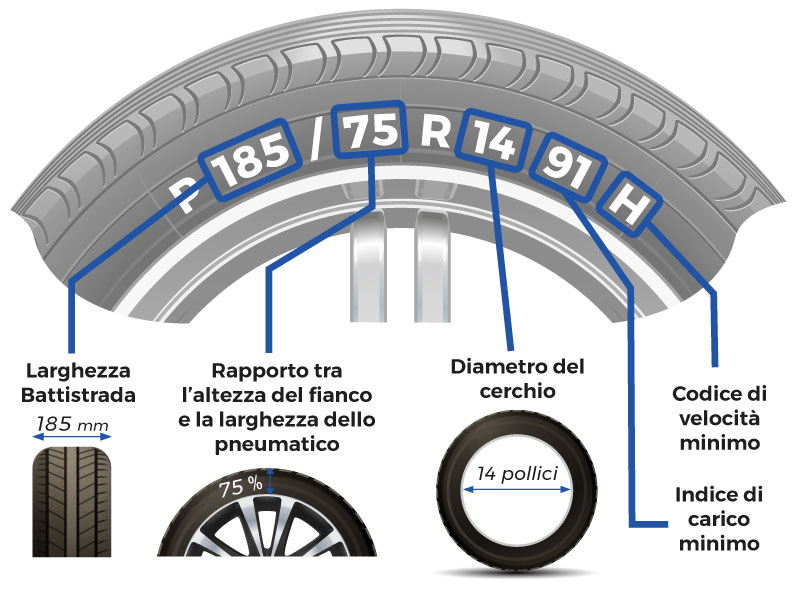
\includegraphics[width=0.7\linewidth]{Figures/tire_measures}
	\caption{Esempio di misure, secondo la notazione ETRTO, riportate sulla spalla dello pneumatico.}
	\label{tiremeasures}
\end{figure}
%
\section{Modelli di pneumatico}
Le forze di contatto tra la superficie stradale e lo pneumatico possono essere descritte da un vettore di forza risultante applicato in un punto specifico dell'impronta di contatto e da una coppia risultante, come illustrato nella \figurename{  \ref{tireforces}}.

\begin{figure}[h!]
	\centering
	\begin{subfigure}{0.4\linewidth}
		$F_x$ \quad forza longitudinale\\
		$F_y$ \quad forza laterale\\
		$F_z$ \quad forza verticale\\
		$T_x$ \quad coppia di sovrasterzo\\
		$T_y$ \quad resistenza al rotolamento\\
		$T_z$ \quad coppia di autoallineamento
	\end{subfigure}
	\begin{subfigure}{0.4\linewidth}
		\centering
		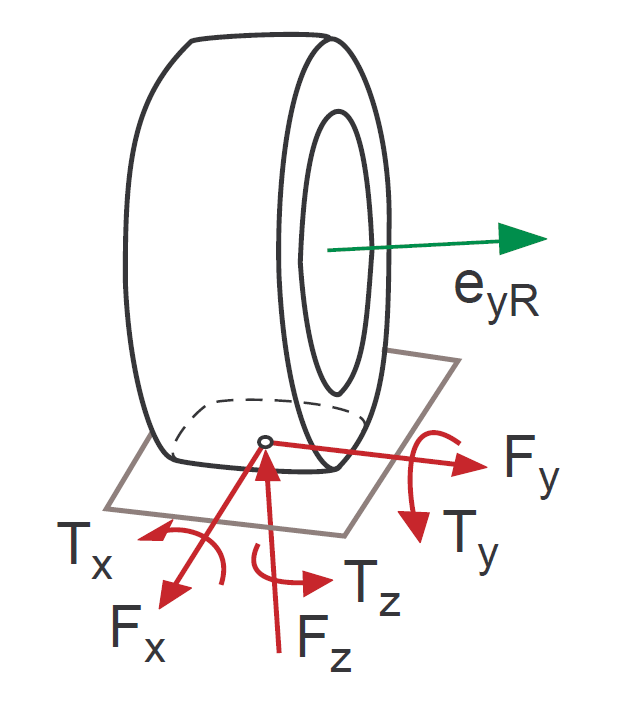
\includegraphics[width=\linewidth]{Figures/tire_forces}
	\end{subfigure}
\caption{Forze e coppie generate dal contatto pneumatico/strada.}
Da: \citeauthor{Rill}, \citetitle{Rill}.
\label{tireforces}
\end{figure}
%
Come componenti cruciali per la movimentazione dei veicoli e il comportamento di guida, le forze degli pneumatici richiedono particolare attenzione soprattutto perché dev'essere considerato anche il comportamento non stazionario. Attualmente, è possibile suddividere i modelli di pneumatico in tre gruppi:
\begin{itemize}
	\item modelli matematici;
	\item modelli fisici;
	\item combinazione dei precedenti.
\end{itemize}
La prima tipologia di modello tenta di rappresentare le caratteristiche fisiche dello pneumatico attraverso una descrizione puramente matematica. Pertanto, questo tipo di modelli parte da un curve caratteristiche ricavate sperimentalmente e cercano di derivare un comportamento approssimativo dall'interpolazione di un grande insieme di dati. Un esempio ben noto di questo approccio è il \textbf{modello di Pacejka} o \textbf{\textit{Magic Formula}} \cite{hans}. Questo tipo di modellazione è adatta per la simulazione di guida in cui il comportamento di interesse è per lo più la manovrabilità del veicolo e le frequenze di uscita sono ben al di sotto delle frequenze di risonanza della cintura dello pneumatico. I modelli fisici o i modelli ad alta frequenza, come i modelli agli elementi finiti, sono in grado di rilevare fenomeni di risonanza a frequenza più elevata. Ciò permette di valutare il comfort di guida di un veicolo. Dal punto di vista del calcolo, i modelli fisici complessi richiedono molto tempo al calcolatore per essere risolti, nonché di molti dati, al contrario dei più veloci modelli matematici, che richiedono un'accurata preelaborazione dei dati sperimentali. La terza tipologia di modelli consiste in un'estensione dei modelli matematici attraverso le leggi fisiche al fine di coprire una gamma di frequenza più ampia.

Il modello di pneumatico sviluppato nel modello di veicolo e il tipo di interfaccia di pneumatico/strada presentato da \citeauthor{Larcher} in \cite{Larcher} si basano sulla \textit{Magic Formula} 6.2.
%
\subsection{Il modello di Pacejka}
Uno dei modelli di pneumatici più utilizzati è il cosiddetto modello \textit{Magic Formula} sviluppato da \citeauthor{bakker} in \cite{bakker}. Questo modello è stato poi rivisto più volte e l'ultima versione è riportata in \cite{hans}. Il modello \textit{Magic Formula} consiste in una pura descrizione matematica del rapporto \textit{input-output} del contatto pneumatico/strada. Questa formulazione collega le variabili di forza con lo \textit{slip} rigido del corpo. La forma generale della funzione può essere scritta come:
%
\begin{equation}
y(x) = D\sin\{C\arctan[B(x + S_h ) - E(B(x + S_h ) - \arctan(B(x + S_h )))]\} + S_v
\end{equation}
%
dove i fattori rappresentano:
\begin{itemize}
	\item $B$ la rigidezza;
	\item $C$ la forma;
	\item $D$ il valore massimo della forza o coppia;
	\item $E$ la curvatura in corrispondenza del valore massimo;
	\item $S_v$ lo spostamento in verticale della curva caratteristica;
	\item $S_h$ lo spostamento in orizzontale della curva caratteristica.
\end{itemize}
e dove $y(x)$ può rappresentare la forza longitudinale $F_x$ , la forza laterale $F_y$ o la coppia di autoallineamento $M_z$, mentre $x$ è la componente di \textit{slip} corrispondente. In \figurename{ \ref{pacejka}} sono illustrate le curve caratteristiche generiche degli pneumatici derivate con il metodo della \textit{Magic Formula}.\\
Per poter utilizzare la \textit{Magic Formula} è necessario conoscere:
\begin{itemize}
	\item la geometria dello pneumatico;
	\item lo slittamento (o \textit{slip});
	\item la forza verticale applicata allo pneumatico;
	\item la penetrazione in corrispondenza del punto di contatto e la sua derivata nel tempo;
	\item l'inclinazione tra piano strada e sistema di riferimento del centro ruota (angolo di camber relativo).
\end{itemize}
È proprio nell'inclinazione tra piano strada e sistema di riferimento del centro ruota che si porrà una maggiore attenzione in quanto elemento fondamentale per ricavare l'effettivo punto di contatto dell'interazione pneumatico/strada.
%
\begin{figure}[h]
	\centering
	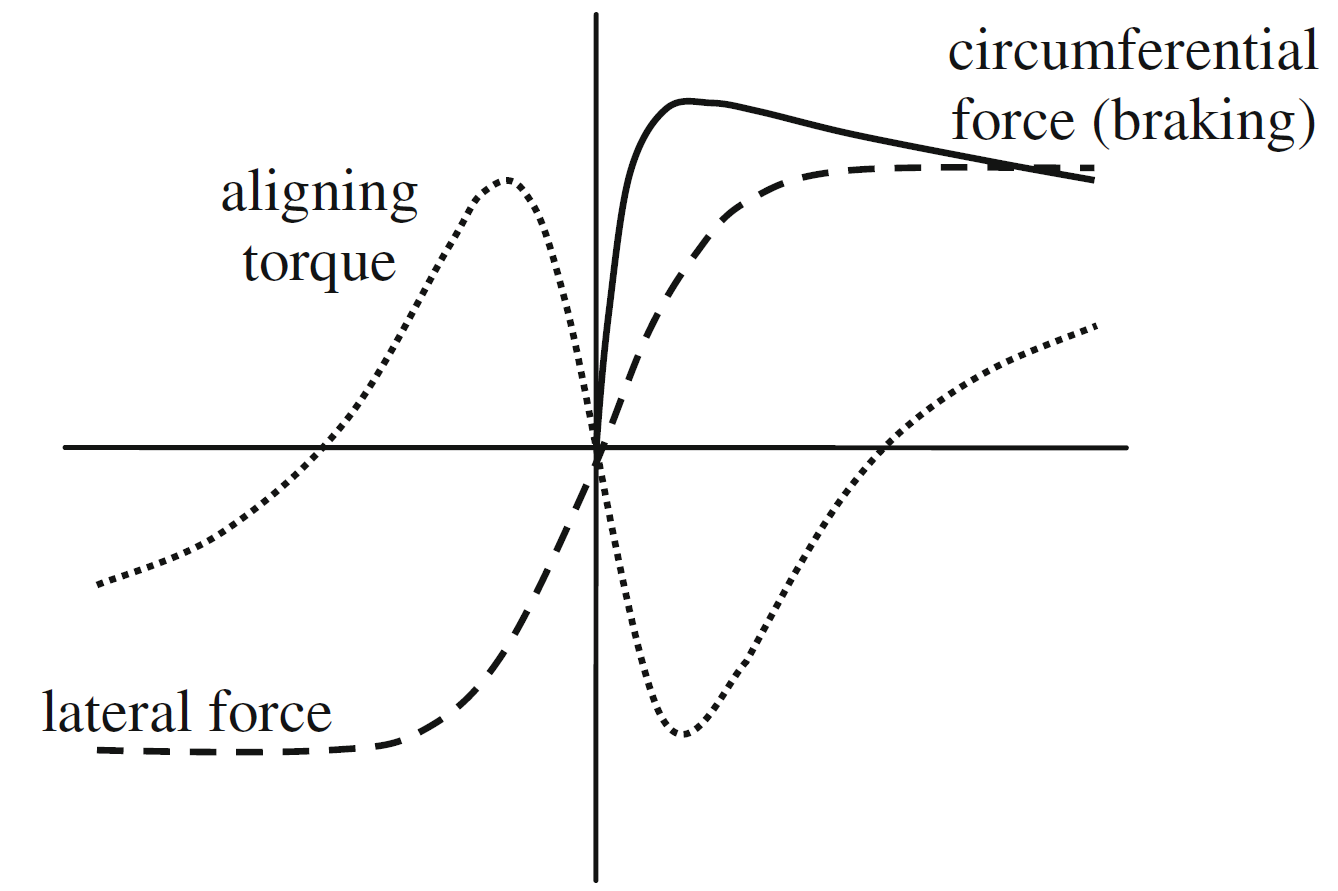
\includegraphics[width=0.58\linewidth]{Figures/pacejka}
	\caption{Curve caratteristiche generiche degli pneumatici derivate con il metodo della \textit{Magic Formula}.}
	Da: \citeauthor{Schramm}, \citetitle{Schramm}.
	\label{pacejka}
\end{figure}
%
\section{Contatto con la superficie stradale}
%
Si analizzeranno ora le quattro metodologie di complessità crescente per ricavare l'inclinazione del piano locale e i punti di contatto sulla superficie stradale $P_{PL}$, nonché sulla circonferenza del disco indeformabile $P_{MF}$ dove effettivamente agiranno le forze ricavate mediante la \textit{Magic Formula}. Dapprima si utilizzerà un metodo a disco singolo presentato in \cite{Rill}, successivamente si passerà ad un modello a più dischi, così da coprire una superficie stradale maggiore e avere quindi risultati più precisi, soprattutto in prossimità di variazioni repentine del manto stradale.
%
\subsection{Modello di pneumatico a disco singolo}
%
\subsubsection{Contatto di Rill}
\label{Contatto_Rill}
%
\paragraph{Piano locale}
La posizione e l'orientamento della ruota in relazione al sistema fissato a terra sono dati dalla terna di riferimento del vettore ruota $RF_{wh}$, che viene calcolata istante per istante risolvendo le equazioni dinamiche del sistema ottenuto nel Capitolo 2 in \cite{Larcher}. Supponendo che il profilo stradale sia rappresentato da una funzione arbitraria a due coordinate spaziali del tipo: 
%
\begin{equation}
z=z(x,y)
\end{equation}
%
su una superficie irregolare, il punto di contatto con il piano locale $P_{PL}$ non può essere calcolato direttamente. Nel metodo a disco singolo presentato in \cite{Rill} da \citeauthor{Rill}, come prima approssimazione si identifica un punto di contatto $P^\star$ come una semplice traslazione del centro ruota $M$:
%
\begin{equation}
P^\star = M-R_0\textbf{\textit{e}}_{zC}
\begin{bmatrix}
x^\star\\
y^\star\\
z^\star
\end{bmatrix}
\end{equation}
%
dove $R_0$ è il raggio dello pneumatico indeformato ed $\textbf{\textit{e}}_{zC}$ è il vettore unitario che definisce l'asse $z_C$ del sistema di riferimento della ruota.

\begin{figure}[h]
	\centering
	\begin{subfigure}{0.45\linewidth}
		\centering
		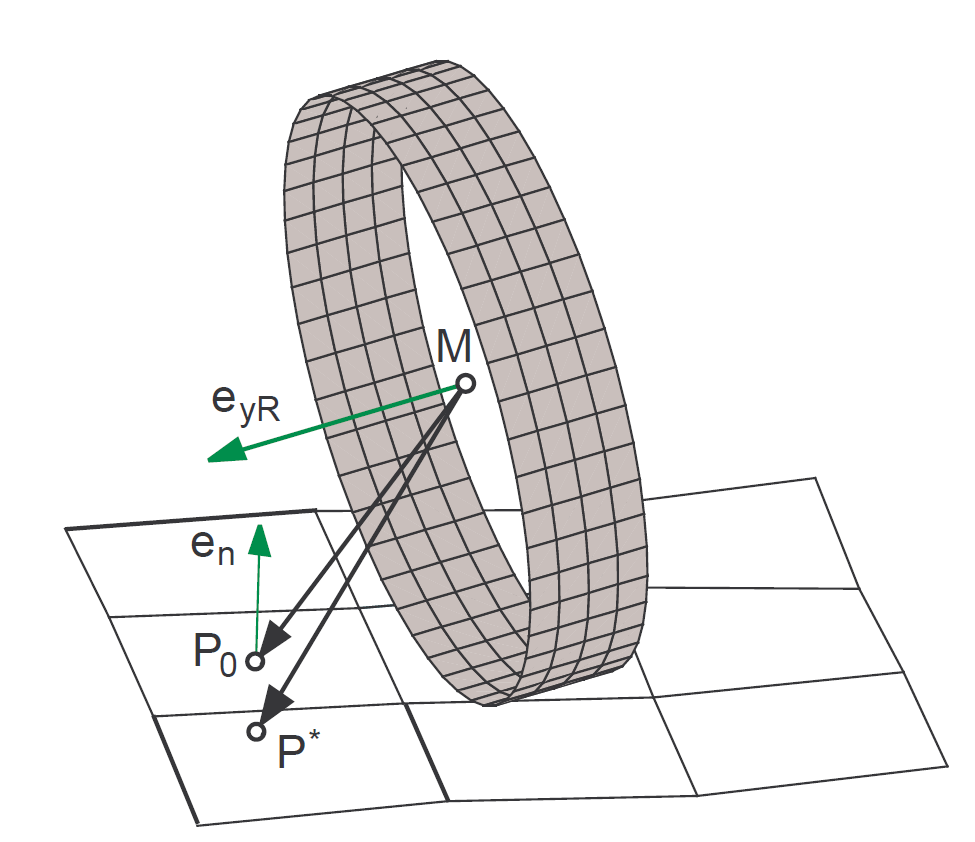
\includegraphics[width=\linewidth]{Figures/contact_geometry_1}
	\end{subfigure}
	\begin{subfigure}{0.35\linewidth}
		\centering
		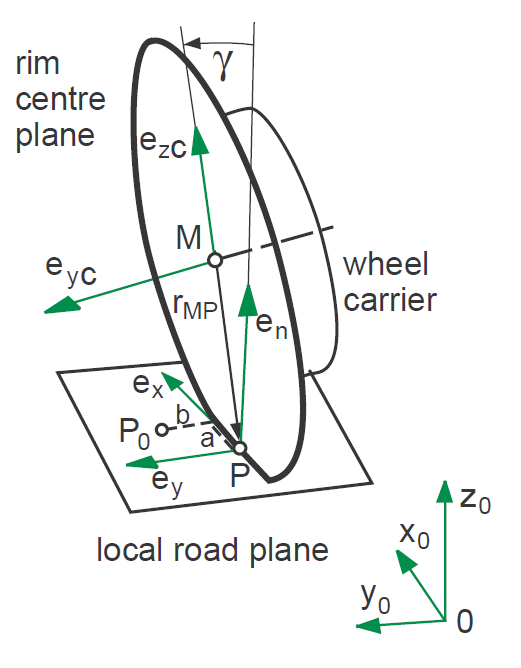
\includegraphics[width=\linewidth]{Figures/contact_geometry_2}
	\end{subfigure}
	\caption{Geometria del contatto pneumatico-strada.}
	Da: \citeauthor{Rill}, \citetitle{Rill}.
	\label{contactgeometry}
\end{figure}

La prima stima del sistema di riferimento del punto di contatto $RF_{P^\star}$ è una terna con origine in $P^\star$ e la medesima orientazione degli assi del sistema di riferimento della ruota. Si noti dunque che l'origine di $RF_{P^\star}$ corrisponde alla proiezione lungo l'asse $z_C$ del sistema di riferimento della ruota.

\begin{equation}
RF_{P^\star} = \left[
\begin{array}{ccc|c}
& & & x^\star\\
\multicolumn{3}{c|}{\multirow{3}{*}{\raisebox{20mm}{\scalebox{1.5}{$[R_{RF_{wh}}]$}}}} & y^\star\\
& & & z^\star\\ \hline
0 & ~~0 & 0 & 1
\end{array}\right]
\end{equation}\\

Al fine di ottenere una buona approssimazione del piano strada locale in termini di inclinazione longitudinale e laterale, sono stati utilizzati i quattro punti di campionamento $(Q^\star_1, Q^\star_2, Q^\star_3, Q^\star_4)$, rappresentati graficamente in \figurename{ \ref{localtrack}}. I punti di campionamento sono definiti nel sistema di riferimento temporaneo del punto di contatto $RF_{P^\star}$; lo spostamento longitudinale e laterale sono definiti dall'origine, ovvero dallo stesso $P^\star$. I vettori di spostamento sono definiti come:
%
\begin{equation}
\begin{split}
\textbf{\textit{r}}_{Q^\star_{1,2}} = \pm \Delta x \textbf{\textit{e}}_{xP^\star} = \pm \Delta x \textbf{\textit{e}}_{xC} \\
\textbf{\textit{r}}_{Q^\star_{3,4}} = \pm \Delta y \textbf{\textit{e}}_{yP^\star} = \pm \Delta y \textbf{\textit{e}}_{yC}
\end{split}
\end{equation}
%
e quindi, i quattro punti di campionamento sono:
%
\begin{equation}
\begin{split}
Q^\star_{1,2} = P^\star \pm \textbf{\textit{r}}_{Q^\star_{1,2}} = P^\star \pm \Delta x \textbf{\textit{e}}_{xC} \\
Q^\star_{3,4} = P^\star \pm \textbf{\textit{r}}_{Q^\star_{3,4}} = P^\star \pm \Delta y \textbf{\textit{e}}_{yC}
\end{split}
\end{equation}
%
Al fine di campionare il terreno nel modo più efficace possibile, le distanze di $\Delta x$ e $\Delta y$, dell'equazione precedente, vengono regolate in base al raggio indeformato $R_0$ e alla larghezza $B$ dello pneumatico. I valori di queste due quantità possono essere trovate in \cite{Rill} e sono $\Delta x = 0.1 R_0$ e $\Delta x = 0.3 B$. Attraverso questa definizione, si può ottenere un comportamento sufficientemente realistico durante la simulazione.

\begin{figure}[h]
	\centering
	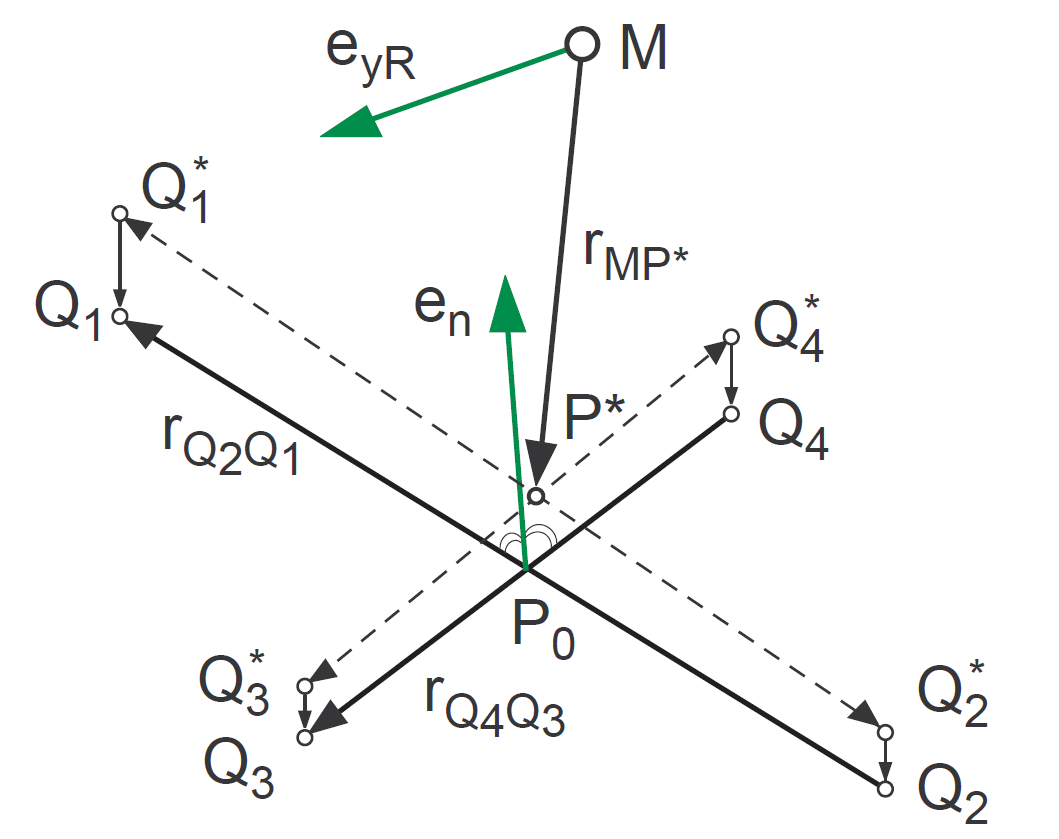
\includegraphics[width=0.5\linewidth]{Figures/local_track}
	\caption{Punti campionati nel piano locale della superficie stradale.}
	Da: \citeauthor{Rill}, \citetitle{Rill}.
	\label{localtrack}
\end{figure}

Ora, la componente $z$ in corrispondenza dei quattro punti campione, viene valutata attraverso la funzione $z(x,y)$ precedentemente definita. Quindi, aggiornando la terza coordinata dei punti di campionamento $Q^\star_i$, si ottengono i corrispondenti punti campione $Q_i$ sulla superficie. La linea fissata dai punti $Q_1$, $Q_2$ e $Q_3$, $Q_4$, può ora essere utilizzata per definire la normale al piano strada locale (\figurename{ \ref{localplane}}). Pertanto, il vettore normale è definito come:
%
\begin{equation}
\textbf{\textit{e}}_n = \frac{\textbf{\textit{r}}_{Q_1 Q_2} \times \textbf{\textit{r}}_{Q_4 Q_3}}{|\textbf{\textit{r}}_{Q_1 Q_2} \times \textbf{\textit{r}}_{Q_4 Q_3}|}
\label{normale}
\end{equation}
%
Ora, i versori $\textbf{\textit{e}}_x$ ed $\textbf{\textit{e}}_y$, che descrivono l'inclinazione del piano locale nel possono essere ottenuti dalle seguenti equazioni:
%
\begin{equation}
\textbf{\textit{e}}_x = \frac{\textbf{\textit{e}}_{yC}\times\textbf{\textit{e}}_{n}}{|\textbf{\textit{e}}_{yC}\times\textbf{\textit{e}}_{n}|}
\qquad
\textbf{\textit{e}}_{y} = \textbf{\textit{e}}_{n}\times\textbf{\textit{e}}_{x}
\label{terna}
\end{equation}
%
dove sono $\textbf{\textit{r}}_{Q_2 Q_1}$ e $\textbf{\textit{r}}_{Q_4 Q_3}$ sono i vettori che puntano rispettivamente da $Q_1$ a $Q_2$ e da $Q_3$ a $Q_4$. Applicando la \eqref{terna} è ora possibile calcolare i vettori unitari $\textbf{\textit{e}}_{x}$ e $\textbf{\textit{e}}_{y}$ del piano locale di contatto. Per definire univocamente il piano strada, oltre alla normale calcolata in \eqref{normale}, viene utilizzato il punto $P_n$ dato dal valore medio delle tre coordinate spaziali dei quattro punti campione.
%
\begin{equation}
P_n = \frac{1}{4}\begin{bmatrix}
\sum_{i=1}^{4} x_i \\
\sum_{i=1}^{4} y_i \\
\sum_{i=1}^{4} z_i
\end{bmatrix}
\end{equation}
%
\paragraph{Punti di contatto}
\label{Punti_contatto_rill}
Infine, è necessario ricondursi alle condizioni tali per cui il modello di Pacejka è valido trovando il punto di contatto sul piano strada locale $P_{PL}$ e il punto di contatto sulla circonferenza del disco indeformabile $P_{MF}$ dove effettivamente agiranno le forze ricavate mediante la \textit{Magic Formula}. Si troverà dapprima la componente della normale al piano strada $\textbf{\textit{e}}_{n_{XZ}}$ sul piano in cui giace il singolo disco indeformabile. $P_{MF}$ sarà dunque trovato a partire dal centro ruota $M$, moltiplicando scalarmente il versore $-\textbf{\textit{e}}_{n_{XZ}}$ per il raggio del disco indeformabile $R_0$, ovvero:
%
\begin{equation}
P_{MF} = -R_0\textbf{\textit{e}}_{n_{XZ}}
\label{puntoMF}
\end{equation}
%
Come illustrato in \figurename{ \ref{localplane}}, il punto di contatto sul piano strada locale $P_{PL}$ viene invece calcolato sfruttando un algoritmo di intersezione piano-raggio (che si tratterà nel Capitolo \ref{Geom_Algos}). $P_{PL}$ giacerà dunque sulla proiezione in direzione $-\textbf{\textit{e}}_{n_{XZ}}$ del punto $M$ sulla retta individuata dal punto $P_n$ e normale $\textbf{\textit{e}}_{n_{XZ}}$.

\begin{figure}[h]
	\centering
	\hfill
	% TO DO: sistemare normale al piano strada, non coerente con il disegno
	\begin{subfigure}{.49\textwidth}
		\centering
		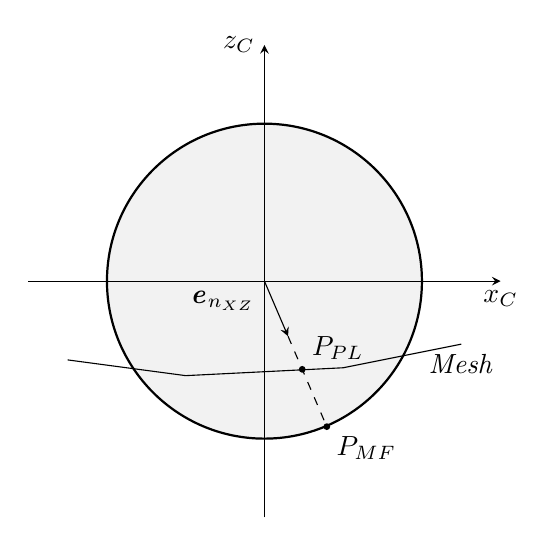
\begin{tikzpicture}
		\def\axisl{3};
		\def\zd{1.9};
		\draw[thick, fill=gray!10] (0,0) circle (2);
		\draw[-stealth] (-\axisl,0) -- (\axisl,0) node[below]{$x_C$};
		\draw[-stealth] (0,-\axisl) -- (0,\axisl) node[left]{$z_C$};
		\draw[] (-2.5,-1)  -- (-1,-1.2) -- (1,-1.1) -- (2.5,-0.8) node[below]{\textit{Mesh}};
		\draw[fill] (2.5,-0.8);
		\draw[-stealth] (0,0) node[below left]{$\textbf{\textit{e}}_{n_{XZ}}$} -- (0.3,-0.7)  ;
		\draw[dashed] (0.3,-0.7) -- (0.3*2.64,-0.7*2.64)  ;
		\draw[fill] (0.3*2.64,-0.7*2.64) circle [radius=1pt] node[below right]{$P_{MF}$};
		\draw[fill] (0.3*1.6,-0.7*1.6) circle [radius=1pt] node[above right]{$P_{PL}$};
		\end{tikzpicture}
	\end{subfigure}
	\hfill
	\begin{subfigure}{.49\textwidth}
		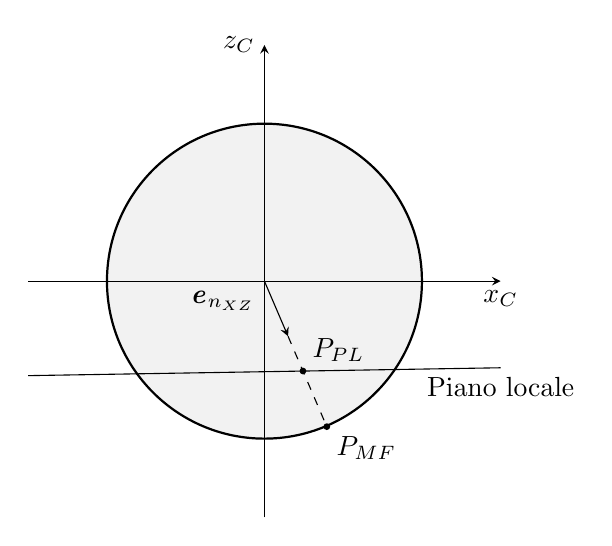
\begin{tikzpicture}
		\def\axisl{3};
		\def\zd{1.9};
		\draw[thick, fill=gray!10] (0,0) circle (2);
		\draw[-stealth] (-\axisl,0) -- (\axisl,0) node[below]{$x_C$};
		\draw[-stealth] (0,-\axisl) -- (0,\axisl) node[left]{$z_C$};
		\draw[] (-3,-1.2) -- (3,-1.1) node[below]{Piano locale};
		\draw[fill] (2.5,-0.8);
		\draw[-stealth] (0,0) node[below left]{$\textbf{\textit{e}}_{n_{XZ}}$} -- (0.3,-0.7)  ;
		\draw[dashed] (0.3,-0.7) -- (0.3*2.64,-0.7*2.64)  ;
		\draw[fill] (0.3*2.64,-0.7*2.64) circle [radius=1pt] node[below right]{$P_{MF}$};
		\draw[fill] (0.3*1.63,-0.7*1.63) circle [radius=1pt] node[above right]{$P_{PL}$};
		\end{tikzpicture}
	\end{subfigure}
	\hfill
	\caption{Punti di contatto $P_{PL}$ e $P_{MF}$ in relazione alla normale $\textbf{\textit{e}}_{n_{XZ}}$ e al tipo di terreno.}
	\label{localplane}
\end{figure}

Infine si possono unire tutte le componenti del piano di riferimento del punto di contatto $P_{MF}$ ottenendo il relativo sistema di riferimento:
%
\begin{equation}
RF_{MF} = \left[
\begin{array}{ccc|c}
& & & x_{P_{MF}}\\
\multirow{3}{*}{\raisebox{20mm}{\scalebox{1.5}{$\left[\textbf{\textit{e}}_x\right]$}}} & \multirow{3}{*}{\raisebox{20mm}{\scalebox{1.5}{$\left[\textbf{\textit{e}}_y\right]$}}} & \multirow{3}{*}{\raisebox{20mm}{\scalebox{1.5}{$\left[\textbf{\textit{e}}_z\right]$}}} & y_{P_{MF}}\\
& & & z_{P_{MF}}\\ \hline
0 & 0 & 0 & 1
\end{array}\right]
\end{equation}\\
Attraverso questo approccio, la normale del piano strada locale $\textbf{\textit{e}}_{n}$ insieme al punto di contatto sul piano strada locale $P_{PL}$ e al punto di contatto sulla circonferenza del disco indeformabile $P_{MF}$, sono in grado di rappresentare l'irregolarità della strada in modo soddisfacente ma approssimativo, infatti, bordi taglienti o discontinuità del manto stradale saranno involontariamente filtrate da questo approccio.

Nel caso specifico di questo lavoro la superficie stradale non è rappresentata da una funzione del tipo $z(x,y)$ ma da una serie di triangoli. Questo comporta l'impossibilità di valutare la terza coordinata dei punti di campionamento $Q_i^\star$. Per sopperire a questo problema si utilizzerà l'algoritmo per l'intersezione tra raggio e triangolo presentato nel Capitolo \ref{Geom_Algos}. Si definiranno dunque i punti di origine dei raggi direttamente nel sistema di riferimento della ruota $RF_{wh}$ come:
\begin{equation}
\begin{split}
Q^\star_{1,2} = M \pm \textbf{\textit{r}}_{Q^\star_{1,2}} = P^\star \pm \Delta x \textbf{\textit{e}}_{xC} \\
Q^\star_{3,4} = M \pm \textbf{\textit{r}}_{Q^\star_{3,4}} = P^\star \pm \Delta y \textbf{\textit{e}}_{yC}
\end{split}
\end{equation}
dai quali partiranno con direzione $-z_C$ e intersecheranno la \textit{mesh} nei punti $(Q_1, Q_2, Q_3, Q_4)$.
%
\subsubsection{Contatto ponderato in base all'area d'intersezione}
%
\paragraph{Piano locale}
In alternativa, si può utilizzare un modello di contatto ponderato in base all'area di intersezione. In altre, parole si andrà a valutare triangolo per triangolo l'intersezione con il disco indeformabile. Prima di tutto si intersecherà il triangolo nello spazio con il piano in cui giace il disco trovando dunque un segmento. Successivamente si valuterà l'intersezione di questo segmento con il disco, calcolando l'area tra il segmento stesso e il semicerchio inferiore del disco.

\begin{figure}
	\centering
	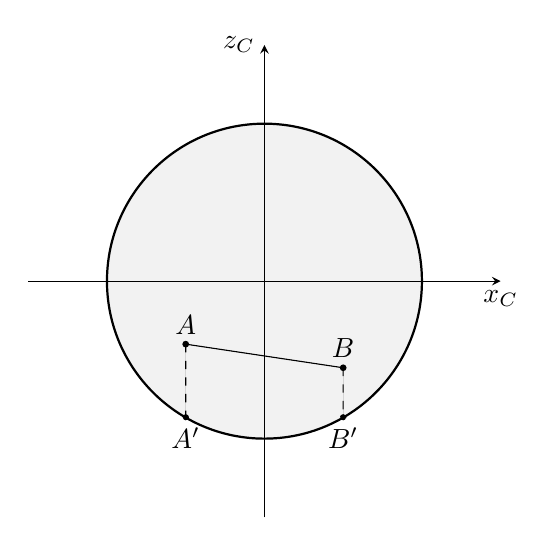
\begin{tikzpicture}
	\def\axisl{3};
	\def\zd{1.9};
	\draw[thick, fill=gray!10] (0,0) circle (2);
	\draw[-stealth] (-\axisl,0) -- (\axisl,0) node[below]{$x_C$};
	\draw[-stealth] (0,-\axisl) -- (0,\axisl) node[left]{$z_C$};
	\draw[fill] (-1,-0.8) circle [radius=1pt] node[above]{$A$} --  (1,-1.1) circle [radius=1pt] node[above]{$B$};
	\draw[dashed, fill] (-1,-0.8) --  (-1,-2*0.866) circle [radius=1pt] node[below]{$A'$};
	\draw[dashed, fill] (1,-1.1) --  (1,-2*0.866) circle [radius=1pt] node[below]{$B'$};	
	\end{tikzpicture}
	\caption{Dato un generico triangolo che, intersecando il piano in cui giace il disco, crea il segmento dato dai punti $A$ e $B$, l'area di intersezione è la regione racchiusa dai segmenti $B'B$, $AB$, $AA'$ e dall'arco di circonferenza $A'B'$.}
\end{figure}
\begin{figure}
	\centering
	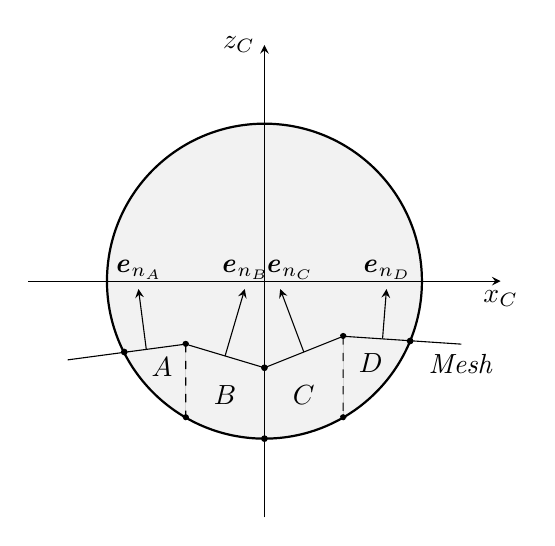
\begin{tikzpicture}
	\def\axisl{3};
	\def\zd{1.9};
	\draw[thick, fill=gray!10] (0,0) circle (2);
	\draw[-stealth] (-\axisl,0) -- (\axisl,0) node[below]{$x_C$};
	\draw[-stealth] (0,-\axisl) -- (0,\axisl) node[left]{$z_C$};
	\draw[] (-2.5,-1)  -- (-1,-0.8) --  (0,-1.1) -- (1,-0.7) -- (2.5,-0.8) node[below]{\textit{Mesh}};
	\draw[fill] (0,-1.1) circle [radius=1pt];
	\draw[fill] (0,-2) circle [radius=1pt];
	\draw[fill] (-1.78,-0.9) circle [radius=1pt];
	\draw[fill] (1.85,-0.76) circle [radius=1pt];
	\draw[dashed, fill] (-1,-0.8)  circle [radius=1pt] --  (-1,-2*0.866)  circle [radius=1pt];
	\draw[dashed, fill] (1,-0.7)  circle [radius=1pt] --  (1,-2*0.866)  circle [radius=1pt];
	\draw[]  (1.35,-0.8) node[below]{$D$};
	\draw[]  (0.5,-1.2) node[below]{$C$};
	\draw[]  (-0.5,-1.2) node[below]{$B$};
	\draw[]  (-1.3,-0.85) node[below]{$A$};
	\draw[-stealth] (1.5,-0.73) -- (1.55,-0.1) node[above]{$\textbf{\textit{e}}_{n_D}$};
	\draw[-stealth] (0.5,-0.9)  -- (0.2,-0.1) node[above]{$~~\textbf{\textit{e}}_{n_C}$};
	\draw[-stealth] (-0.5,-0.95) -- (-0.25,-0.1) node[above]{$\textbf{\textit{e}}_{n_B}$};
	\draw[-stealth] (-1.5,-0.87) -- (-1.6,-0.1) node[above]{$\textbf{\textit{e}}_{n_A}$};
	\end{tikzpicture}
	\caption{I versori normali $\textbf{\textit{e}}_{n_A}$, $\textbf{\textit{e}}_{n_B}$, $\textbf{\textit{e}}_{n_C}$ e $\textbf{\textit{e}}_{n_D}$ vengono ponderati in base all'area delle rispettive regioni d'intersezione $A$, $B$, $C$ e $D$.}
\end{figure}

Attraverso questa area si potrà pesare la normale alla faccia del triangolo considerato e quindi effettuare una media ponderata con tutti gli atri triangoli che intersecano il disco, ovvero:
%
\begin{equation}
\textbf{\textit{e}}_n = \sum_{i=0}^{N_T}A_i\textbf{\textit{e}}_{n_i}
\label{ponderata}
\end{equation}
%
dove:
\begin{itemize}
	\item $N_T$ è il numero di triangoli all'interno della \ac{BB} rappresentante l'ombra dello pneumatico;
	\item $\textbf{\textit{e}}_n$ è il versore normale risultante;
	\item $\textbf{\textit{e}}_{n_i}$ è il versore normale dell'$i$-esimo triangolo;
	\item $A_i$ corrisponde all'area tra il segmento creato dall'intersezione piano-triangolo e il semicerchio inferiore del disco dell'$i$-esimo triangolo.
\end{itemize}

Questo metodo è ovviamente utilizzabile solo nel caso di strada rappresentata tramite \textit{mesh} triangolare. A differenza dal modello di \cite{Rill}, permette di non approssimare la superficie stradale mediante soli quattro punti invece di avere una rappresentazione che sfrutta tutti i dati messi a disposizione dalla discretizzazione del manto stradale.
%
\paragraph{Punti di contatto}
Per trovare il punto di contatto con la \textit{mesh} $P_{PL}$ e il punto di contatto sulla circonferenza del disco indeformabile $P_{MF}$ precedentemente definiti, si andrà a ripetere l'operazione in \ref{Punti_contatto_rill} per trovare la componente della normale al piano strada $\textbf{\textit{e}}_{n_{XZ}}$ sul piano in cui giace il singolo disco indeformabile. A differenza del modello di contatto di Rill, non si ha ora una definizione univoca del piano strada locale. Infatti, l'unica componente ad ora conosciuta è il versore risultante normale al terreno $\textbf{\textit{e}}_n$. Per ricavare il punto di contatto sulla circonferenza del disco indeformabile $P_{MF}$ si utilizzerà la \eqref{puntoMF}, mentre per il punto sulla \textit{mesh} $P_{PL}$ si andrà ad utilizzare un algoritmo d'intersezione tra raggio e la superficie stradale, dove l'origine del raggio sarà il centro ruota e la direzione $-\textbf{\textit{e}}_{n_{XZ}}$.
%
\subsection{Modello di pneumatico a più dischi}
%
In questo modello lo pneumatico sarà rappresentato da più dischi rigidi indeformabili disposti uniformemente lungo la sezione dello stesso. Essi potranno avere raggio uguale o diverso l'uno dall'altro, in modo da rappresentare una forma specifica dello pneumatico.
%
\begin{figure}[h!]
	\hfill
	\begin{subfigure}{.3\textwidth}
		\centering
		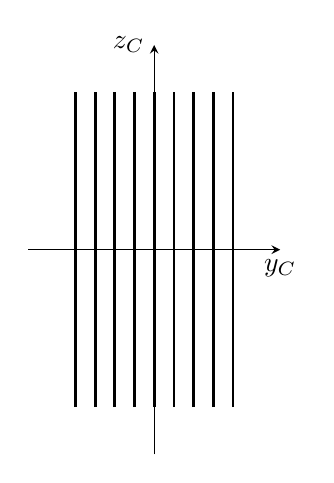
\begin{tikzpicture}
		\def\axisl{2};
		\def\zd{1};
		\draw[-stealth] (-0.8*\axisl,0) -- (0.8*\axisl,0) node[below]{$y_C$};
		\draw[-stealth] (0,-1.3*\axisl) -- (0,1.3*\axisl) node[left]{$z_C$};
		
		\draw[line width=0.35mm] (-1,-\axisl/\zd) -- (-1,\axisl/\zd);
		\draw[line width=0.35mm] (-0.75,-\axisl/\zd) -- (-0.75,\axisl/\zd);
		\draw[line width=0.35mm] (-0.5,-\axisl/\zd) -- (-0.5,\axisl/\zd);
		\draw[line width=0.35mm] (-0.25,-\axisl/\zd) -- (-0.25,\axisl/\zd);
		
		\draw[line width=0.35mm] (0,-\axisl/\zd) -- (0,\axisl/\zd);

		\draw[line width=0.35mm] (0.25,-\axisl/\zd) -- (0.25,\axisl/\zd);
		\draw[line width=0.35mm] (0.5,-\axisl/\zd) -- (0.5,\axisl/\zd);
		\draw[line width=0.35mm] (0.75,-\axisl/\zd) -- (0.75,\axisl/\zd);
		\draw[line width=0.35mm] (1,-\axisl/\zd) -- (1,\axisl/\zd);
		\end{tikzpicture}
		\caption{Raggio uniforme}
	\end{subfigure}
	\hfill
	\begin{subfigure}{.3\textwidth}
		\centering
		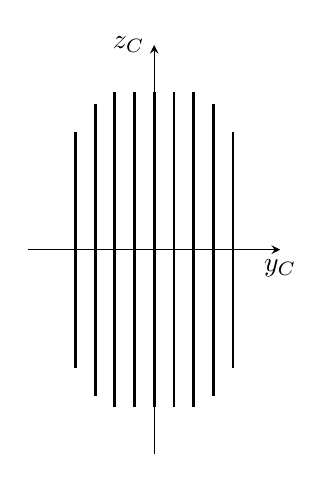
\begin{tikzpicture}
		\def\axisl{2};
		\def\zd{1};
		\draw[-stealth] (-0.8*\axisl,0) -- (0.8*\axisl,0) node[below]{$y_C$};
		\draw[-stealth] (0,-1.3*\axisl) -- (0,1.3*\axisl) node[left]{$z_C$};
		
		\draw[line width=0.35mm] (-1,-\axisl/\zd+0.5) -- (-1,\axisl/\zd-0.5);
		\draw[line width=0.35mm] (-0.75,-\axisl/\zd+0.5-0.5*1.41/2) -- (-0.75,\axisl/\zd-0.5+0.5*1.41/2);
		\draw[line width=0.35mm] (-0.5,-\axisl/\zd) -- (-0.5,\axisl/\zd);
		\draw[line width=0.35mm] (-0.25,-\axisl/\zd) -- (-0.25,\axisl/\zd);
		
		\draw[line width=0.35mm] (0,-\axisl/\zd) -- (0,\axisl/\zd);
		
		\draw[line width=0.35mm] (0.25,-\axisl/\zd) -- (0.25,\axisl/\zd);
		\draw[line width=0.35mm] (0.5,-\axisl/\zd) -- (0.5,\axisl/\zd);
		\draw[line width=0.35mm] (0.75,-\axisl/\zd+0.5-0.5*1.41/2) -- (0.75,\axisl/\zd-0.5+0.5*1.41/2);
		\draw[line width=0.35mm] (1,-\axisl/\zd+0.5) -- (1,\axisl/\zd-0.5);
		\end{tikzpicture}
		\caption{Spalla raccordata}
	\end{subfigure}
	\hfill
		\begin{subfigure}{.3\textwidth}
		\centering
		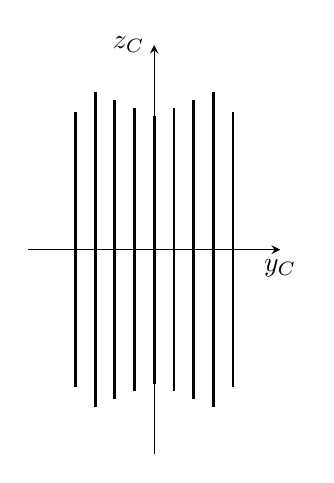
\begin{tikzpicture}
		\def\axisl{2};
		\def\zd{1};
		\draw[-stealth] (-0.8*\axisl,0) -- (0.8*\axisl,0) node[below]{$y_C$};
		\draw[-stealth] (0,-1.3*\axisl) -- (0,1.3*\axisl) node[left]{$z_C$};
		
		\draw[line width=0.35mm] (-1,-\axisl/\zd+0.25) -- (-1,\axisl/\zd-0.25);
		\draw[line width=0.35mm] (-0.75,-\axisl/\zd) -- (-0.75,\axisl/\zd);
		\draw[line width=0.35mm] (-0.5,-\axisl/\zd+0.1) -- (-0.5,\axisl/\zd-0.1);
		\draw[line width=0.35mm] (-0.25,-\axisl/\zd+0.2) -- (-0.25,\axisl/\zd-0.2);
		
		\draw[line width=0.35mm] (0,-\axisl/\zd+0.3) -- (0,\axisl/\zd-0.3);
		
		\draw[line width=0.35mm] (0.25,-\axisl/\zd+0.2) -- (0.25,\axisl/\zd-0.2);
		\draw[line width=0.35mm] (0.5,-\axisl/\zd+0.1) -- (0.5,\axisl/\zd-0.1);
		\draw[line width=0.35mm] (0.75,-\axisl/\zd) -- (0.75,\axisl/\zd);
		\draw[line width=0.35mm] (1,-\axisl/\zd+0.25) -- (1,\axisl/\zd-0.25);
		\end{tikzpicture}
		\caption{Profilo personalizzato}
	\end{subfigure}
	\hfill
	\caption{Disposizione dei dischi.}
\end{figure}

Anche se questo modello di pneumatico è costituito da più dischi, il punto di contatto $P_{MF}$ utilizzato per valutare la formula di Pacejka verrà comunque considerato nel disco fittizio giacente sul piano $XZ$ dello pneumatico. Equivalentemente, anche il punto di contatto con la \textit{mesh} $P_{PL}$ verrà considerato nel medesimo piano.

\begin{figure}[h!]
	\centering
	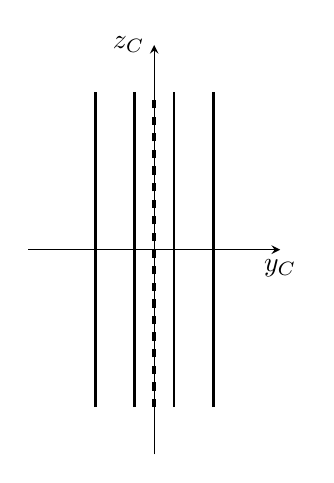
\begin{tikzpicture}
	\def\axisl{2};
	\def\zd{1};
	\draw[-stealth] (-0.8*\axisl,0) -- (0.8*\axisl,0) node[below]{$y_C$};
	\draw[-stealth] (0,-1.3*\axisl) -- (0,1.3*\axisl) node[left]{$z_C$};
	
	\draw[line width=0.35mm] (-0.75,-\axisl/\zd) -- (-0.75,\axisl/\zd);
	\draw[line width=0.35mm] (-0.25,-\axisl/\zd) -- (-0.25,\axisl/\zd);
	\draw[dashed, line width=0.5mm] (0,-\axisl/\zd) -- (0,\axisl/\zd);
	\draw[line width=0.35mm] (0.25,-\axisl/\zd) -- (0.25,\axisl/\zd);
	\draw[line width=0.35mm] (0.75,-\axisl/\zd) -- (0.75,\axisl/\zd);
	\end{tikzpicture}
	\caption{Pneumatico rappresentato da dischi a raggio uniforme. Notare il disco fittizio giacente sul piano $XZ$ in linea tratteggiata.}
\end{figure}

\begin{figure}[h!]
	\hfill
	\begin{subfigure}{.49\linewidth}
	\centering
	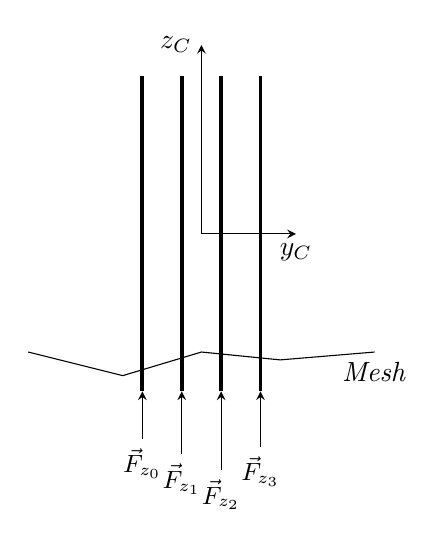
\begin{tikzpicture}
		\def\axisl{2};
		\def\zd{1};
		\draw[-stealth] (0,0) -- (0.6*\axisl,0) node[below]{$y_C$};
		\draw[-stealth] (0,0) -- (0,1.2*\axisl) node[left]{$z_C$};
		
		\draw[line width=0.5mm] (-0.75,-\axisl/\zd) -- (-0.75,\axisl/\zd);
		\draw[line width=0.5mm] (-0.25,-\axisl/\zd) -- (-0.25,\axisl/\zd);
		\draw[line width=0.5mm] (0.25,-\axisl/\zd) -- (0.25,\axisl/\zd);
		\draw[line width=0.5mm] (0.75,-\axisl/\zd) -- (0.75,\axisl/\zd);
		
		\draw[] (-2.2,-1.5) -- (-1,-1.8) --  (0,-1.5) -- (1,-1.6) -- (2.2,-1.5) node[below]{\textit{Mesh}};
		
		\draw[-stealth] (0.75,-\axisl/\zd-0.7) node[below]{\small$\vec{F}_{z_3}$} -- (0.75,-\axisl/\zd);
		\draw[-stealth] (0.25,-\axisl/\zd-1) node[below]{\small$\vec{F}_{z_2}$} -- (0.25,-\axisl/\zd);
		\draw[-stealth] (-0.25,-\axisl/\zd-0.8) node[below]{\small$\vec{F}_{z_1}$} -- (-0.25,-\axisl/\zd);
		\draw[-stealth] (-0.75,-\axisl/\zd-0.6) node[below]{\small$\vec{F}_{z_0}$} -- (-0.75,-\axisl/\zd);
	\end{tikzpicture}
	\end{subfigure}
\hfill
	\begin{subfigure}{.49\linewidth}
	\centering
	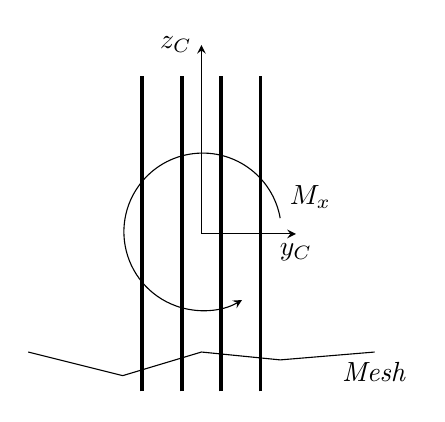
\begin{tikzpicture}
		\def\axisl{2};
		\def\zd{1};
		\draw[-stealth] (0,0) -- (0.6*\axisl,0) node[below]{$y_C$};
		\draw[-stealth] (0,0) -- (0,1.2*\axisl) node[left]{$z_C$};
		
		\draw[line width=0.5mm] (-0.75,-\axisl/\zd) -- (-0.75,\axisl/\zd);
		\draw[line width=0.5mm] (-0.25,-\axisl/\zd) -- (-0.25,\axisl/\zd);
		\draw[line width=0.5mm] (0.25,-\axisl/\zd) -- (0.25,\axisl/\zd);
		\draw[line width=0.5mm] (0.75,-\axisl/\zd) -- (0.75,\axisl/\zd);
		
		\draw[-stealth] (1,0.2) node[above right]{$M_x$} arc (10:300:1) ;
		
		\draw[] (-2.2,-1.5) -- (-1,-1.8) --  (0,-1.5) -- (1,-1.6) -- (2.2,-1.5) node[below]{\textit{Mesh}};
	\end{tikzpicture}
	\end{subfigure}
\hfill
\caption{Momento creato dalla morfologia del terreno.}
\end{figure}
%
\subsubsection{Contatto ponderato in base all'area d'intersezione}
\paragraph{Piano locale}
Analogamente al modello di pneumatico a singolo disco, si può effettuare la stessa operazione su ogni disco per trovare il versore normale risultante $\textbf{\textit{e}}_{n_{D_j}}$ relativo al contatto del $j$-esimo disco. La \eqref{ponderata} diventerà dunque:
%
\begin{equation}
\textbf{\textit{e}}_{n_{D_j}} = \sum_{i=0}^{N_T}A_i\textbf{\textit{e}}_{n_i}
\end{equation}
%
Per combinare assieme i versori normali $\textbf{\textit{e}}_{n_{D_j}}$ relativi ai dischi si effettuerà una nuova media ponderata pesata questa volta sull'area totale d'intersezione all'interno del disco. La formula sarà dunque:
%
\begin{equation}
\textbf{\textit{e}}_n = \sum_{j=0}^{N_D}A_{D_j}\textbf{\textit{e}}_{n_{D_j}}
\end{equation}
%
dove:
\begin{itemize}
	\item $N_D$ è il numero di dischi totali rappresentanti lo pneumatico;
	\item $\textbf{\textit{e}}_n$ è il versore normale risultante;
	\item $\textbf{\textit{e}}_{n_{D_j}}$ è il versore normale associato al $j$-esimo disco;
	\item $A_{D_j}$ corrisponde all'area d'intersezione all'interno del $j$-disco e sotto la superficie della \textit{mesh}.
\end{itemize}
\begin{figure}
	\centering
	\tdplotsetmaincoords{70}{110}
	\tdplotsetrotatedcoords{90}{90}{0}
	\begin{tikzpicture}[tdplot_main_coords]
	
	\draw[-stealth] (0,0,0) -- (8,0,0) node[anchor=north east]{$x_C$};
	\draw[-stealth] (0,0,0) -- (0,3,0) node[anchor=north west]{$y_C$};
	\draw[-stealth] (0,0,0) -- (0,0,5) node[anchor=north west]{$z_C$};
	
	\def\r{4};
	\draw[-stealth] (0,1.6,-\r+0.5) -- (0,1.6,-\r+1.5);
	\draw[-stealth] (0,1.2,-\r+0.5-0.5*1.41/2) -- (0-0.1,1.2+0.1,-\r+1.5-0.5*1.41/2);
	\draw[-stealth] (0,0.8,-\r) -- (0,0.8,-\r+1);
	\draw[-stealth] (0,0.4,-\r) -- (0+0.1,0.4-0.1,-\r+1);
	\draw[-stealth] (0,0,-\r) -- (0+0.05,0-0.1,-\r+1);
	\draw[-stealth] (0,-0.4,-\r) -- (0,-0.4,-\r+1);
	\draw[-stealth] (0,-0.8,-\r) -- (0+0.1,-0.8+0.1,-\r+1);
	\draw[-stealth] (0,-1.2,-\r+0.5-0.5*1.41/2) -- (0,-1.2,-\r+1.5-0.5*1.41/2);
	\draw[-stealth] (0,-1.6,-\r+0.5) -- (0,-1.6,-\r+1.5);
	
	\begin{scope}[tdplot_rotated_coords]
	\tdplotdrawarc[tdplot_rotated_coords,thick]{(0,0,1.6)}{\r-0.5}{0}{360}{}{}
	
	\tdplotdrawarc[tdplot_rotated_coords,thick]{(0,0,1.2)}{\r-0.5+0.5*1.41/2}{3}{-228}{}{}
	\tdplotdrawarc[tdplot_rotated_coords, dashed,thick]{(0,0,1.2)}{\r-0.5+0.5*1.41/2}{3}{360-228}{}{}
	
	\tdplotdrawarc[tdplot_rotated_coords,thick]{(0,0,0.8)}{\r}{-9}{-217}{}{}
	\tdplotdrawarc[tdplot_rotated_coords, dashed,thick]{(0,0,0.8)}{\r}{-9}{360-217}{}{}
	
	\tdplotdrawarc[tdplot_rotated_coords,thick]{(0,0,0.4)}{\r}{-15}{-210}{}{}
	\tdplotdrawarc[tdplot_rotated_coords, dashed,thick]{(0,0,0.4)}{\r}{-15}{360-210}{}{}
	
	\tdplotdrawarc[tdplot_rotated_coords,thick]{(0,0,0)}{\r}{-15}{-210}{}{}
	\tdplotdrawarc[tdplot_rotated_coords, dashed,thick]{(0,0,0)}{\r}{-15}{360-210}{}{}
	
	\tdplotdrawarc[tdplot_rotated_coords,thick]{(0,0,-0.4)}{\r}{-15}{-210}{}{}
	\tdplotdrawarc[tdplot_rotated_coords, dashed,thick]{(0,0,-0.4)}{\r}{-15}{360-210}{}{}
	
	\tdplotdrawarc[tdplot_rotated_coords,thick]{(0,0,-0.8)}{\r}{-15}{-210}{}{}
	\tdplotdrawarc[tdplot_rotated_coords, dashed,thick]{(0,0,-0.8)}{\r}{-15}{360-210}{}{}
	
	\tdplotdrawarc[tdplot_rotated_coords,thick]{(0,0,-1.2)}{\r-0.5+0.5*1.41/2}{-17}{-205}{}{}
	\tdplotdrawarc[tdplot_rotated_coords, dashed,thick]{(0,0,-1.2)}{\r-0.5+0.5*1.41/2}{-17}{360-205}{}{}
	
	\tdplotdrawarc[tdplot_rotated_coords,thick]{(0,0,-1.6)}{\r-0.5}{-30}{-195}{}{}
	\tdplotdrawarc[tdplot_rotated_coords, dashed,thick]{(0,0,-1.6)}{\r-0.5}{-20}{360-195}{}{}
	\end{scope}
	\end{tikzpicture}
	\caption{Normali associate ai vari dischi dello pneumatico.}
\end{figure}

\paragraph{Punti di contatto}
Avendo ora a disposizione il versore normale risultante $\textbf{\textit{e}}_n$, si possono trovare i punti $P_{MF}$ e $P_{PL}$ adottando il medesimo metodo utilizzato in \ref{Contatto_Rill}. Si noti che anche se lo pneumatico è rappresentato da più dischi, per ricondursi alle condizioni tali per cui il modello di Pacejka è valido, è necessario immaginare che ci sia sempre un disco fittizio giacente sul piano $XZ$ della ruota.
%
\subsubsection{Contatto tramite campionamento}
\paragraph{Piano locale}
Nel caso in cui la densità della \textit{mesh} sia troppo alta, effettuare il calcolo per il modello di contatto ponderato in base all'area d'intersezione precedentemente presentato, può essere molto dispendioso in termini di calcoli, e quindi di tempo. Per sopperire a questo problema, se il numero di triangoli è superiore ad una certa misura, si andrà a campionare la \textit{mesh} triangolare in corrispondenza del piano in cui giacciono i dischi. In particolare, per campionare la \textit{mesh} si sfrutterà l'algoritmo di intersezione tra raggio e triangolo che verrà presentato nel Capitolo \ref{Geom_Algos}. Attraverso questo algoritmo, supponendo che il raggio abbia la stessa direzione dell'asse $z_C$, si andranno a memorizzare le normali alle facce dei triangoli campionati. Il versore normale risultante $\textbf{\textit{e}}_n$ non verrà più calcolato mediante una media ponderata ma bensì attraverso una semplice media aritmetica tra tutti i punti campionati lungo il disco.

\begin{figure}
	\centering
	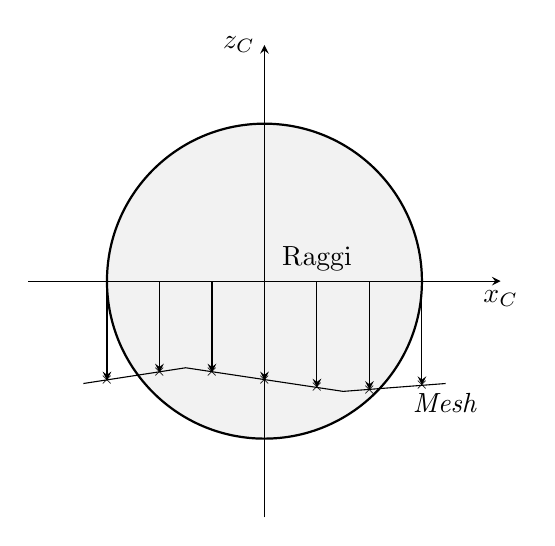
\begin{tikzpicture}
	\def\axisl{3};
	\def\zd{3.5};
	\draw[thick, fill=gray!10] (0,0) circle (2);
	\draw[-stealth] (-\axisl,0) -- (\axisl,0) node[below]{$x_C$};
	\draw[-stealth] (0,-\axisl) -- (0,\axisl) node[left]{$z_C$};
	\draw[-stealth] (-2,0) -- (-2,-1.26) node[]{\tiny$\times$};
	\draw[-stealth] (2,0) -- (2,-1.32) node[]{\tiny$\times$};
	\draw[-stealth] (-2*2/3,0) -- (-2*2/3,-1.16) node[]{\tiny$\times$};
	\draw[-stealth] (2*2/3,0) -- (2*2/3,-1.38) node[]{\tiny$\times$};
	\draw[-stealth] (-2/3,0) -- (-2/3,-1.16) node[]{\tiny$\times$};
	\draw[-stealth] (2/3,0) node[above]{Raggi} -- (2/3,-1.35) node[]{\tiny$\times$};
	\draw[-stealth] (0,0) -- (0,-1.26) node[]{\tiny$\times$};
	\draw[] (-2.3,-1.3) -- (-1,-1.1) --  (1,-1.4) -- (2.3,-1.3) node[below]{\textit{Mesh}};
	\end{tikzpicture}
	\caption{Campionamento della \textit{mesh} triangolare in corrispondenza del piano in cui giace l'$i$-esimo disco. I raggi partono dall'asse $x_C$ in direzione $z_C$.}
\end{figure}

\paragraph{Punti di contatto}
Avendo ora a disposizione il versore normale risultante $\textbf{\textit{e}}_n$, si possono trovare i punti $P_{MF}$ e $P_{PL}$ adottando il medesimo metodo utilizzato in \ref{Contatto_Rill}, sempre tenendo conto che entrambi i punti giaceranno sul disco fittizio corrispondente al piano $XZ$ della ruota. 